% 2014 湖南卷（文）第19题：平面四边形 ABCD
% 条件：DA⊥AB，DE=1，EA=2，∠ADC=2π/3，∠BEC=π/3
% 由条件精确计算：D=(0,3)、E=(0,2)、A=(0,0)、C=(√3,4)、B=(6√3,0)，按 0.8cm/单位
% 全局数值坐标，12pt，.6pt，灰度
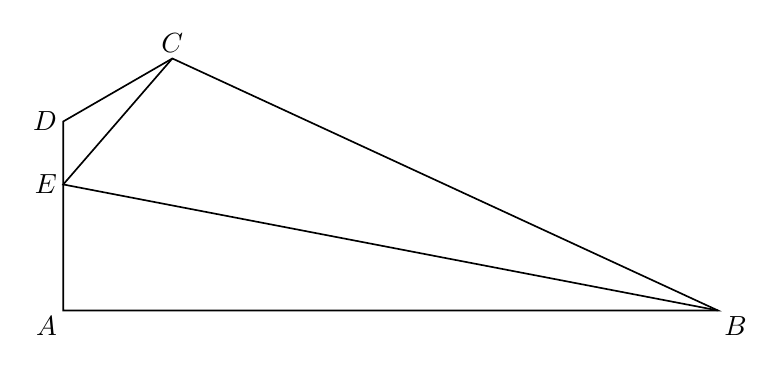
\begin{tikzpicture}[x=1cm,y=1cm,line width=.6pt,
  geometry edge/.style={solid,line width=.6pt},
  geometry label/.style={font=\normalsize,inner sep=2pt}]
\coordinate (A) at (0,0);
\coordinate (E) at (0,1.6);
\coordinate (D) at (0,2.4);
\coordinate (C) at (1.3856,3.2);
\coordinate (B) at (8.3138,0);
\draw[geometry edge] (A)--(B)--(C)--(D)--cycle;
\draw[geometry edge] (C)--(E)--(B);
\node[geometry label,below left] at (A) {$A$};
\node[geometry label,below right] at (B) {$B$};
\node[geometry label,above] at (C) {$C$};
\node[geometry label,left] at (D) {$D$};
\node[geometry label,left] at (E) {$E$};
\end{tikzpicture}
